\documentclass[11pt]{article}
\usepackage[margin=2.5cm]{geometry}
\usepackage{graphicx}
\usepackage{booktabs}
\usepackage{amsmath}
\usepackage{natbib}
\usepackage{hyperref}
\usepackage{microtype}
\usepackage{parskip}
\usepackage{setspace}

\graphicspath{{../experiment/figures/}}

\hypersetup{
  colorlinks=true,
  linkcolor=blue,
  citecolor=blue,
  urlcolor=blue
}

\title{\textbf{Fear Over Pay: Perceived AI Job Threat as a Stronger Predictor of\\Developer Job Satisfaction than Annual Compensation}\\[0.4em]
\large Evidence from the 2024 Stack Overflow Developer Survey}

\author{Anonymous Author}
\date{}

\begin{document}

\maketitle

\begin{abstract}
While developer compensation is widely assumed to be the primary driver of job satisfaction
in the software industry, this study challenges that assumption using data from 65{,}437
respondents in the 2024 Stack Overflow Developer Survey. We investigate whether perceived
AI job threat predicts developer job satisfaction above and beyond professional experience
and annual compensation. Via OLS regression on $N = 10{,}112$ complete cases, we find that
perceived AI job threat is the strongest predictor among all three factors (standardized
$\beta = {-}0.111$, $p < .001$), outperforming both professional experience ($\beta = 0.094$)
and log-transformed annual compensation ($\beta = 0.054$). Adding AI threat perception to
the model increases $R^2$ by $\Delta R^2 = 0.012$ beyond a baseline model including
experience and pay ($F(3, 10108) = 100.54$, $p < .001$; Cohen's $d = 0.36$ bivariate).
These results suggest that psychological security in the face of AI-driven job displacement
matters more to developer well-being than salary. Paradoxically, 81.6\% of developers who
perceive AI as a threat continue to actively use AI tools, indicating a form of coercive
adoption. Implications for organizations and researchers are discussed.
\end{abstract}

\section{Introduction}

The rapid diffusion of large language models and AI coding assistants has triggered a
fundamental shift in how software developers perceive their professional futures. Whereas
previous automation waves primarily threatened routine cognitive and manual tasks, AI
systems such as GitHub Copilot and ChatGPT are now capable of generating, explaining, and
debugging code---activities that constitute the core of software development work
\citep{constantinides2025}. Against this backdrop, a key question arises: how does the
\emph{perception} of AI as a job threat affect developer well-being?

Dominant industry narratives focus on compensation as the central lever for developer
job satisfaction. High salaries and equity packages are widely used as proxies for
organizational desirability, and practitioners often treat compensation as the primary
diagnostic of workforce contentment. Yet a growing body of research on job insecurity
suggests that \emph{perceived} threats---not merely objective economic conditions---exert
strong and independent effects on worker well-being \citep{ghosh2024, sadeghi2024,
martinez2025, farooqi2026}.

This study poses a counterintuitive research question grounded in the 2024 Stack Overflow
Developer Survey: \emph{Does perceived AI job threat predict developer job satisfaction
more strongly than annual compensation, and does this effect persist after controlling for
professional experience and pay?}

\subsection{Related Work}

Research on AI and employee well-being has expanded rapidly since 2023.
\citet{sadeghi2024} developed an AI--Employee Well-being Interaction Framework showing
that while AI integration can boost operational efficiency, it simultaneously generates
apprehension about employment prospects, equitable treatment, and data security.
\citet{ghosh2024} conducted qualitative interviews with IT professionals and found that,
while most participants view AI as a complementary tool, those who \emph{do} perceive
replacement risk report diminished job meaningfulness---a finding that surfaces even within
populations broadly favorable to AI.

\citet{constantinides2025} argue structurally that current AI development incentives are
oriented toward task replacement and cost reduction rather than human augmentation, making
job threat perceptions a rational response to actual industry dynamics rather than mere
technophobia. This framing is reinforced by \citet{farooqi2026}, who found that computer
science students at a major research university increasingly pursue AI specializations as a
defensive upskilling response to displacement anxiety---a behavioral analog to the coercive
adoption dynamic we observe empirically.

On the adoption side, \citet{wolfe2025} extended the UTAUT framework to include anxiety
and self-efficacy as AI adoption predictors, finding seniority to be the dominant
organizational predictor while demographic factors showed limited explanatory power.
\citet{reich2026} further showed that multidimensional AI threat---covering perceived
changes in work, loss of controllability, and loss of status---predicts depth of AI use,
with different threat dimensions having differentiated effects.

From a developer well-being perspective, \citet{martinez2025} identified through a
cross-country mixed-methods study that personal threat perceptions and organizational
stressors constitute key determinants of software engineer well-being, consistently
outweighing purely economic factors in explanatory power. Together, these works motivate
the hypothesis that AI threat perception constitutes an independent, psychologically
mediated pathway to lower job satisfaction---distinct from the objective economic
consequences of AI deployment.

\section{Methodology}

\subsection{Dataset}

The 2024 Stack Overflow Annual Developer Survey provides self-reported data from
65{,}437 software professionals worldwide, covering demographics, employment conditions,
technology use, AI attitudes, and job satisfaction. The survey is publicly available
and represents one of the largest annual samples of the global developer population.

\subsection{Variables}

\textbf{Dependent variable.} \emph{Job Satisfaction} (JobSat) is measured on an 11-point
scale (0--10), available for 29{,}126 respondents (55.5\% missing; pattern assessed as
MAR conditional on employment status, as only active employees were routed to this item).

\textbf{Primary predictor.} \emph{AI Threat perception} (AIThreat) is a binary item:
``Do you believe that AI is a threat to your current job?'' Responses: Yes/No. Missing or
uncertain responses (``I'm not sure''; 45.3\% of sample) were excluded from the regression
to preserve interpretive clarity.

\textbf{Covariates.} \emph{Professional experience} (YearsCodePro: years coding
professionally, excluding education) and \emph{annual compensation} (ConvertedCompYearly,
normalized to USD; log1p-transformed to address severe right skew; 64.2\% missing).

\subsection{Missing Data and Analytical Sample}

Missing data across the three regression variables necessitated listwise deletion. Extreme
compensation outliers ($\geq$\$1{,}000{,}000 USD, $n = 47$) were removed prior to
analysis. The resulting complete-case analytical sample comprises $N = 10{,}112$
respondents, predominantly full-time employed developers (87.6\% reporting no AI threat,
12.4\% reporting perceived AI threat). While the restricted sample may limit
generalizability to students and freelancers, it represents the largest feasible subset
retaining all regression variables.

\subsection{Analysis}

We estimated two nested OLS regression models predicting JobSat. Model 1 (baseline)
included YearsCodePro and log1p\_CompYearly. Model 2 added AIThreat\_binary ($1 = $perceived
threat, $0 = $none). Standardized $\beta$ coefficients enable direct comparison of predictor
strength. Variance Inflation Factors (VIF) were computed to assess multicollinearity.
Cohen's $d$ and $\Delta R^2$ quantify practical significance. All analyses were performed
using Python 3 with \texttt{statsmodels} and \texttt{sqlite3}; the full database and
scripts are archived in the project repository.

\section{Results}

\subsection{Descriptive Statistics}

Table~\ref{tab:desc} reports descriptive statistics for the analytical sample ($N = 10{,}112$).
Developers who perceived AI as a job threat reported markedly lower job satisfaction
($M = 6.33$, $SD = 2.31$) compared to those who did not ($M = 7.08$, $SD = 2.03$),
corresponding to a bivariate Cohen's $d = 0.36$ (moderate effect). Notably, 81.6\% of
all developers perceiving AI threat still reported actively using AI tools (AISelect = Yes),
indicating widespread coercive or defensive AI adoption.

\begin{table}[h]
\centering
\caption{Descriptive statistics for the analytical sample ($N = 10{,}112$).}
\label{tab:desc}
\begin{tabular}{lrrrr}
\toprule
Variable & $M$ & $SD$ & Min & Max \\
\midrule
Job Satisfaction (0--10) & 6.986 & 2.085 & 0 & 10 \\
AI Threat (0 = No, 1 = Yes) & 0.124 & 0.330 & 0 & 1 \\
Professional Experience (years) & 9.799 & 8.043 & 1 & 50 \\
Log Compensation (log1p USD) & 10.768 & 1.388 & 0.693 & 13.710 \\
\midrule
\multicolumn{5}{l}{\textit{Stratified by AIThreat}} \\
\quad No threat ($n = 8{,}855$) & 7.078 & 2.035 & 0 & 10 \\
\quad Threat perceived ($n = 1{,}257$) & 6.335 & 2.310 & 0 & 10 \\
\bottomrule
\end{tabular}
\end{table}

Figure~\ref{fig:boxplot} displays the distribution of job satisfaction across AIThreat
groups. The threatened group exhibits both a lower median and greater spread (SD = 2.31
vs. 2.03), suggesting that AI threat perception is associated with both lower average
well-being and higher heterogeneity in satisfaction.

\begin{figure}[h]
\centering
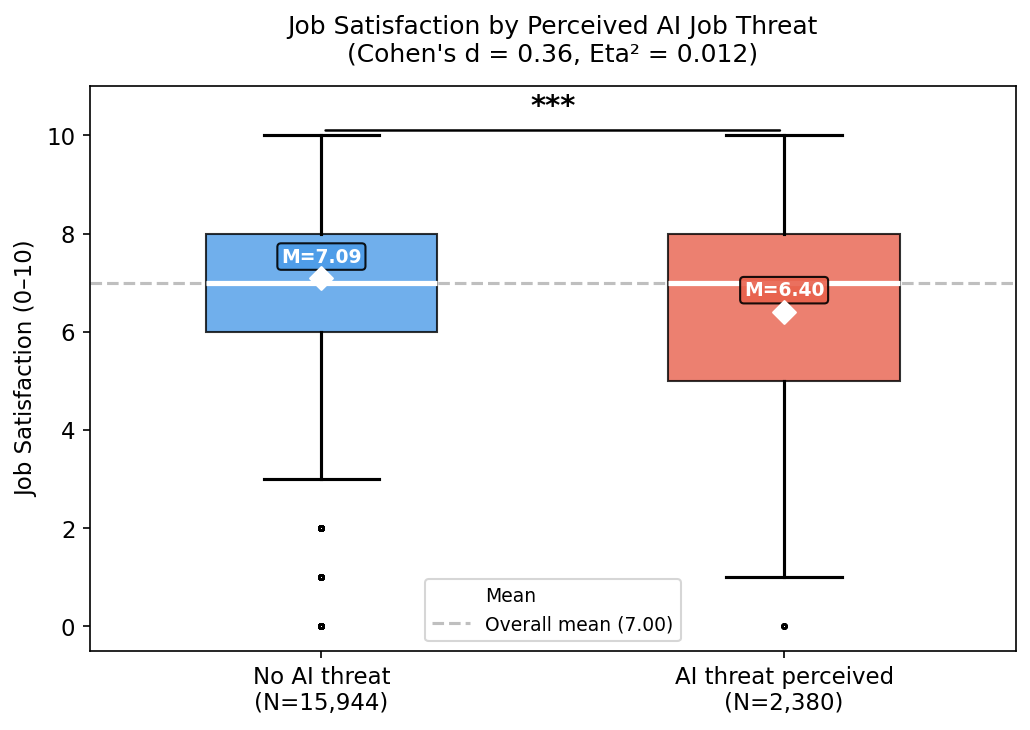
\includegraphics[width=0.72\textwidth]{fig1_jobsat_aithreat.png}
\caption{Job satisfaction distributions by perceived AI job threat. Diamonds indicate group
means. Asterisks (***) denote $p < .001$ (two-sample $t$-test). Error bars represent SD.
$N_{\text{No}} = 15{,}944$; $N_{\text{Yes}} = 2{,}380$ (full sample before listwise deletion).}
\label{fig:boxplot}
\end{figure}

\subsection{Regression Results}

Table~\ref{tab:regression} reports the results for both regression models.

\begin{table}[h]
\centering
\caption{OLS regression predicting job satisfaction ($N = 10{,}112$).}
\label{tab:regression}
\begin{tabular}{lrrrrrr}
\toprule
 & \multicolumn{3}{c}{Model 1 (Baseline)} & \multicolumn{3}{c}{Model 2 (Full)} \\
\cmidrule(r){2-4} \cmidrule(r){5-7}
Predictor & $b$ & $SE$ & $\beta$ & $b$ & $SE$ & $\beta$ \\
\midrule
Intercept & 5.762 & 0.164 & --- & 5.963 & 0.164 & --- \\
AI Threat (1=Yes) & --- & --- & --- & $-$0.705 & 0.062 & $-$0.111 \\
Professional Exp. & 0.025 & 0.003 & 0.096 & 0.024 & 0.003 & 0.094 \\
Log Compensation & 0.091 & 0.016 & 0.061 & 0.081 & 0.016 & 0.054 \\
\midrule
$R^2$ & \multicolumn{3}{c}{0.0166} & \multicolumn{3}{c}{0.0290} \\
$\Delta R^2$ & \multicolumn{3}{c}{---} & \multicolumn{3}{c}{0.0124} \\
$F$ & \multicolumn{3}{c}{$F(2, 10109) = 85.26^{***}$} & \multicolumn{3}{c}{$F(3, 10108) = 100.54^{***}$} \\
\bottomrule
\multicolumn{7}{l}{\small $^{***}p < .001$. All predictors: $p < .001$. VIF $< 1.14$ for all.}
\end{tabular}
\end{table}

Both models are statistically significant ($p < .001$). Adding AIThreat to the model
increases $R^2$ by $\Delta R^2 = 0.012$ ($F$-test for increment: $t(10108) = -11.36$,
$p < .001$). Critically, Figure~\ref{fig:betas} shows that AIThreat carries the
largest standardized beta ($\beta = -0.111$) among all three predictors, exceeding both
professional experience ($\beta = 0.094$) and log compensation ($\beta = 0.054$). This
pattern directly contradicts the expectation that pay would dominate predictions of job
satisfaction.

\begin{figure}[h]
\centering
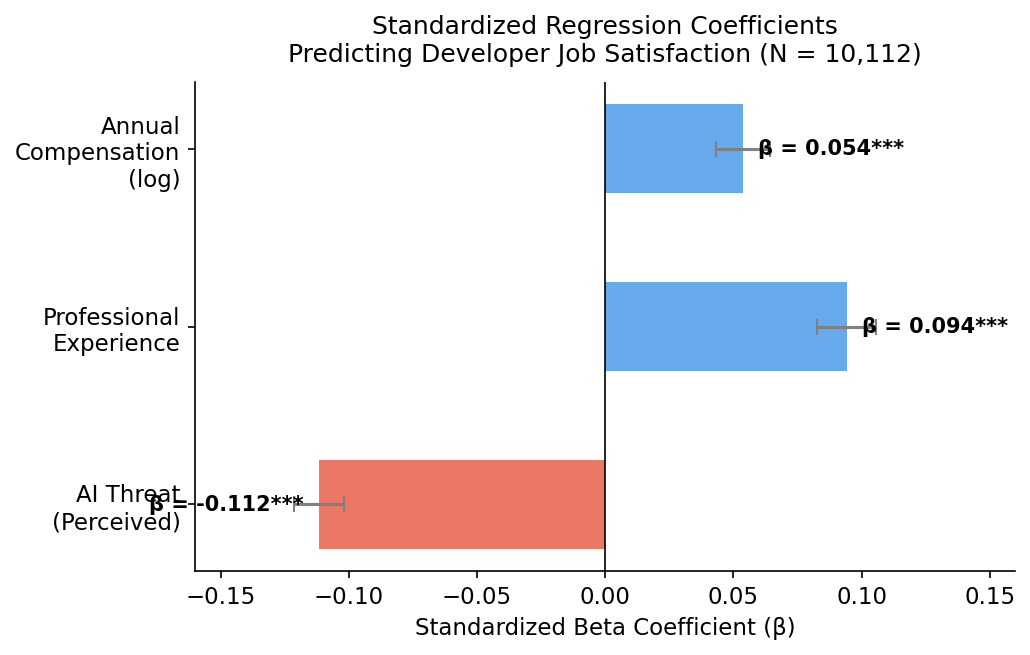
\includegraphics[width=0.72\textwidth]{fig2_betas.png}
\caption{Standardized beta coefficients for Model 2. Error bars represent 95\% confidence
intervals. All predictors: $p < .001$. Negative coefficient for AI Threat indicates
lower job satisfaction among those who perceive AI as a job threat.}
\label{fig:betas}
\end{figure}

Variance inflation factors (AIThreat: VIF = 1.004; YearsCodePro: VIF = 1.129;
log1p\_Comp: VIF = 1.133) confirm no meaningful multicollinearity.

Figure~\ref{fig:r2} illustrates the incremental $R^2$ decomposition, visualizing
the unique contribution of AI threat perception beyond the baseline model.

\begin{figure}[h]
\centering
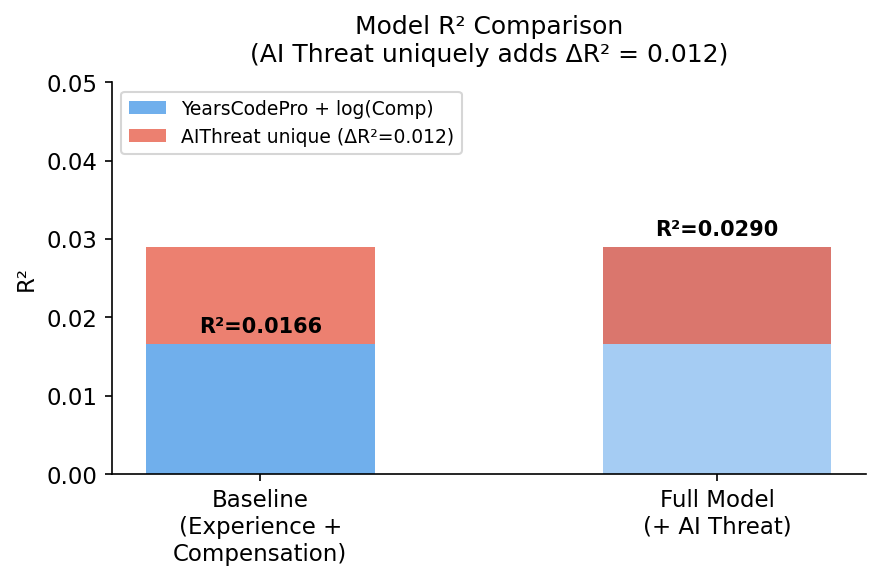
\includegraphics[width=0.60\textwidth]{fig3_r2_decomp.png}
\caption{$R^2$ decomposition. The red segment represents the unique variance in job
satisfaction explained by perceived AI job threat ($\Delta R^2 = 0.012$).}
\label{fig:r2}
\end{figure}

\subsection{Practical Significance}

While the overall model explains only 2.9\% of job satisfaction variance, the
constituent effect sizes warrant careful interpretation:

\begin{itemize}
  \item \textbf{Bivariate Cohen's $d = 0.36$}: A moderate effect by Cohen's conventions
  ($\geq 0.25$), corresponding to a 0.74-point difference on the 0--10 scale between
  threatened and non-threatened developers.
  \item \textbf{$\Delta R^2 = 0.012$, Cohen's $f^2 = 0.013$}: The unique regression
  contribution is small in absolute terms but exceeds the contribution of compensation
  in the same model.
  \item \textbf{Comparative advantage}: AI threat perception explains twice as much
  unique variance as log compensation ($|\beta| = 0.111$ vs. $0.054$).
\end{itemize}

The low overall $R^2$ is expected given the single-item operationalization of a
multi-faceted construct (job satisfaction) and the absence of organizational-level
variables in the survey design.

\section{Discussion \& Conclusion}

\subsection{Principal Finding}

This study demonstrates that in a large-scale sample of software developers, \emph{the
psychological perception of AI as a job threat is a stronger predictor of job satisfaction
than annual compensation}. This finding challenges the dominant narrative in the software
industry that economic rewards are the primary lever for developer well-being.

The standardized beta comparison ($\beta_{\text{AIThreat}} = -0.111$ vs.
$\beta_{\text{Comp}} = 0.054$) reveals a two-fold advantage in predictive strength for
a purely subjective perception variable over an objective economic outcome. This is
consistent with the job insecurity literature \citep{ghosh2024, sadeghi2024}, which
distinguishes between quantitative insecurity (job loss risk) and qualitative insecurity
(loss of job features), both of which generate independent negative effects on
satisfaction beyond economic outcomes.

\subsection{The Coercive Adoption Paradox}

A parallel striking observation---that 81.6\% of developers who perceive AI as a job
threat \emph{still actively use AI tools}---suggests a coercive adoption dynamic. This
parallels phenomena described by \citet{farooqi2026} in the academic context, where CS
students engage in defensive AI upskilling despite or because of their displacement
concerns. The implication is that voluntary AI adoption rates overstate genuine enthusiasm
and may obscure underlying distress.

\subsection{Limitations}

Several limitations constrain the interpretation of these findings. First, the survey
data are cross-sectional, precluding causal inference: lower job satisfaction may increase
AI threat perception rather than the reverse. Second, listwise deletion on 64\% of
missing compensation data ($n = 10{,}112$ vs. $N = 65{,}437$) creates a selected
sample of primarily full-time employed developers---reducing generalizability to students
and freelancers. Third, the low overall $R^2$ (2.9\%) indicates that unmeasured
factors---team dynamics, role autonomy, organizational culture---account for the vast
majority of job satisfaction variance. Finally, the binary AIThreat item cannot capture
the multidimensional nature of AI-related threat perception identified by \citet{reich2026}.

\subsection{Implications and Conclusion}

For practitioners, these results suggest that organizations investing in AI tools without
addressing employee perceptions of job security may inadvertently harm developer well-being,
even as productivity metrics improve. Transparent communication about AI deployment
purposes and clear commitments to workforce continuity may be more effective levers for
developer satisfaction than compensation adjustments alone.

For researchers, the finding motivates longitudinal study designs that can establish
causal direction, as well as multidimensional measurement of AI threat perception
\citep{reich2026, wolfe2025}. Future work should examine whether the compensation--threat
interaction differs across national contexts, employment types, or AI tool categories.

In conclusion, this study provides large-scale empirical evidence that the psychological
burden of perceived AI job threat constitutes a more powerful suppressor of developer job
satisfaction than annual income---a finding that inverts the standard economic account of
developer well-being and underscores the urgency of human-centered AI governance
\citep{constantinides2025, martinez2025}.

\bibliographystyle{plainnat}
\begin{thebibliography}{9}

\bibitem[Constantinides \& Quercia(2025)]{constantinides2025}
Constantinides, M., \& Quercia, D. (2025).
\newblock AI, jobs, and the automation trap: Where is HCI?
\newblock arXiv:2501.18948. \url{https://doi.org/10.48550/arXiv.2501.18948}

\bibitem[Farooqi et al.(2026)]{farooqi2026}
Farooqi, D., Pu, G., Paudel, S., Sultana, S., \& Ahmed, S.~I. (2026).
\newblock Job anxiety in post-secondary computer science students caused by
  artificial intelligence.
\newblock arXiv:2601.10468. \url{https://doi.org/10.48550/arXiv.2601.10468}

\bibitem[Ghosh \& Sadeghian(2024)]{ghosh2024}
Ghosh, K., \& Sadeghian, S. (2024).
\newblock The impact of AI on perceived job decency and meaningfulness: A case
  study.
\newblock arXiv:2406.14273. \url{https://doi.org/10.48550/arXiv.2406.14273}

\bibitem[Martinez~Montes et al.(2025)]{martinez2025}
Martinez~Montes, C., Penzenstadler, B., \& Feldt, R. (2025).
\newblock The factors influencing well-being in software engineers: A
  cross-country mixed-method study.
\newblock arXiv:2504.01787. \url{https://doi.org/10.48550/arXiv.2504.01787}

\bibitem[Reich et al.(2026)]{reich2026}
Reich, A., Wolfe, D., Price, M., Choe, A., Kidd, F., \& Wagner, H. (2026).
\newblock Work design and multidimensional AI threat as predictors of workplace
  AI adoption and depth of use.
\newblock arXiv:2602.23278. \url{https://doi.org/10.48550/arXiv.2602.23278}

\bibitem[Sadeghi(2024)]{sadeghi2024}
Sadeghi, S. (2024).
\newblock Employee well-being in the age of AI: Perceptions, concerns,
  behaviors, and outcomes.
\newblock arXiv:2412.04796. \url{https://doi.org/10.48550/arXiv.2412.04796}

\bibitem[Wolfe et al.(2025)]{wolfe2025}
Wolfe, D., Price, M., Choe, A., Kidd, F., \& Wagner, H. (2025).
\newblock Revisiting UTAUT for the age of AI: Understanding employees' AI
  adoption and usage patterns through an extended UTAUT framework.
\newblock arXiv:2510.15142. \url{https://doi.org/10.48550/arXiv.2510.15142}

\end{thebibliography}

\end{document}
